\documentclass{article}

% \pagenumbering{gobble} % suppress page number
\hyphenchar\font=-1 % suppress hyphenation
\setlength\parindent{0pt} % suppress indentation
\usepackage[margin=1.5truein]{geometry} % set page margins

\usepackage{tikz}
\usetikzlibrary{mindmap}

\usepackage{listings}
\usepackage{fancyhdr}
\usepackage{lastpage}
\usepackage{url}
\usepackage{xcolor}
\usepackage{hyperref}
\usepackage{natbib}

\hypersetup{
    colorlinks = true,
    linkcolor = red,
    urlcolor = red,
    citecolor = black
}

%% page numbering
\pagestyle{fancy}
\fancyhf{}
\fancyfoot[C]{Pg. \thepage \space of \pageref*{LastPage}}
\renewcommand{\headrulewidth}{0pt}

\begin{document}
\title{SYSEN 6000: Foundations of Complex Systems\\~\\
    \Large Mind Mapping \& Emergent Intelligence
}
\author{
    Nick Kunz [NetID: \url{nhk37}] \hyperlink{nhk37@cornell.edu}{nhk37@cornell.edu}}
\date{September 9, 2022}
\maketitle
\thispagestyle{fancy}

\section*{Mind Mapping}
Exhibited below is an illustration of how complex systems could be described by the emergent relationships of their fundamental characteristics. \textit{Note: the systems hierarchy emerges agglomeratively, rather than divisively.}\\

\begin{center}
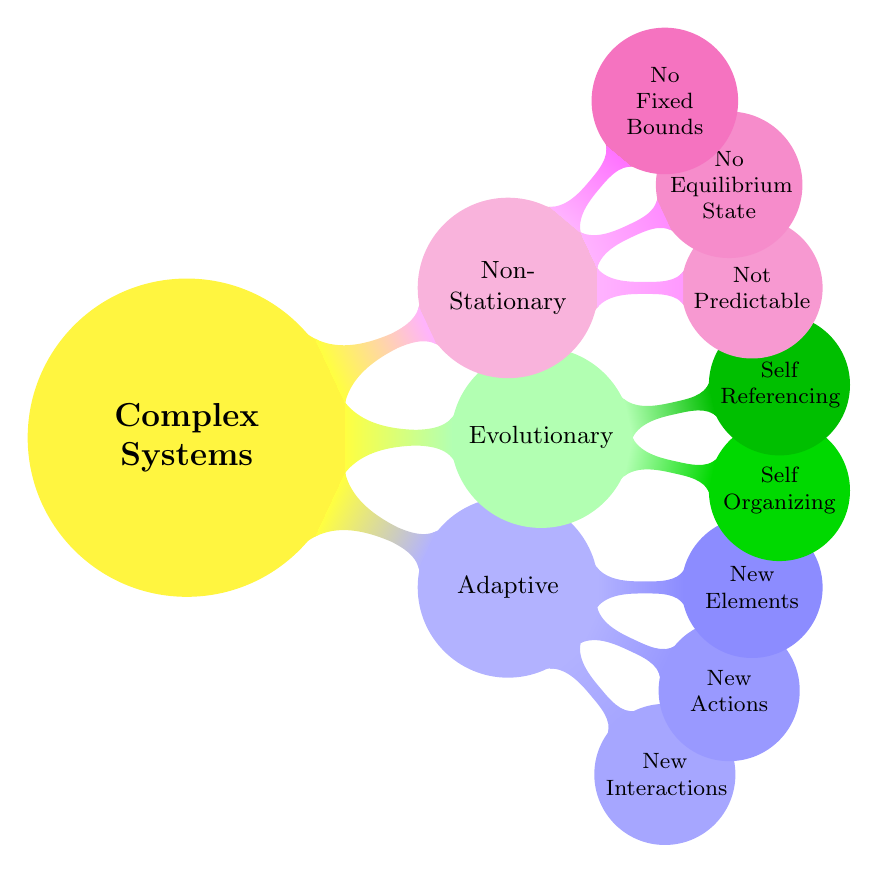
\begin{tikzpicture}[
    mindmap,
    concept color = yellow!75, 
    every node/.style = {concept}, 
    grow cyclic,
    level 1/.append style = {
        level distance = 4.5cm,
        sibling angle = 25
    },
    level 2/.append style = {
        level distance = 3.1cm,
        sibling angle = 25}
]
 
\node{\textbf{Complex Systems}}
    child [concept color = blue!30] {node {Adaptive}
        child [concept color = blue!35] {node {New\\Interactions}}
        child [concept color = blue!40] {node {New\\Actions}}
        child [concept color = blue!45] {node {New\\Elements}}
    }
    child [concept color = green!30] {node {Evolutionary}
        child [concept color = green!85!black] {node {Self\\Organizing}}
        child [concept color = green!75!black] {node {Self\\Referencing}}
    }
    child [concept color = magenta!30] {node {Non-Stationary}
        child [concept color = magenta!40] {node {Not\\Predictable}}
        child [concept color = magenta!45] {node {No\\Equilibrium State}}
        child [concept color = magenta!55] {node {No\\Fixed Bounds}}
    };

\end{tikzpicture}
\end{center}

\newpage
\section*{Emergent Intelligence}

\textit{How does intelligence emerge from non-intelligent components?}\\

The emergence of intelligence from non-intelligent components relies heavily on how we define intelligence. There are many ways we could describe it and the topic is still subject to much debate. However, it is important that we at least get a sense of the range of working definitions. The Merriam-Webster dictionary defines intelligence firstly as \textit{``the ability to learn or understand or to deal with new or trying situations.''} \cite{dictionary} Other definitions take on a scientific view that intelligence is formed through a phenomena that arises strictly from neurological activity in the brain. \cite{brain} There are also theological definitions, which arise from a type of spiritual presence that's met through the mind, body, and soul. \cite{theology} Even with no clear consensus on exactly what intelligence is, it is still possible to reliably assume that we can identify it, when we perceive it.\\

It's possible to observe intelligence on its own. For example, we know that each individual has their own intelligence independent from others, broadly speaking. However, that still doesn't account for how every individual intelligence emerged. Attempting to explain it in material terms - to some extent - begins at the subatomic level, where the evidence for intelligence is weak. \cite{atomic} However, we know interactions are occurring at every level of analysis in order for it to emerge. \cite{info}\cite{origin} In other words, intelligence depends on the \textit{interaction} of non-intelligent components. We might also say that because those interactions are mostly stable, they're largely \textit{algorithmic}, but not necessarily deterministic according to contemporary physics. In that regard, they'd appear more \textit{stochastic}. \cite{random} Here we have a setting where the emergence of intelligence is interactive, algorithmic, and stochastic.\\

It stands to reason that many systems could be described as intelligent, if characterized by the qualities just mentioned. For example, the modern day internet is in fact networked, algorithmic, and stochastic, yet not quite what we'd describe as intelligent. This brings us back to the original question \textit{"How does intelligence emerge from non-intelligent components?"} The last and perhaps the most important quality of intelligence might be the ability to self reference. If we observe our own intelligence, its obvious that we're able to do this. However, an even stricter criteria of self reference might extend all the way into empathy \cite{empathy}. In this sense, it's much more difficult to describe how exactly intelligence emerges from non-intelligent components.\\

We may never be able to fully describe the way(s) in which intelligence emerges. We may also never even reach a consensus on how to define intelligence. However, what we can say is that intelligence is certainly complex. Furthermore, that the complexity we observe exists within a complex system of components. Perhaps by better understanding complex systems with better developed theory and practice, we might better understand intelligence, as it seems best described at a systems level of analysis. It warrants serious consideration that intelligence might not be understood in any other way. The systems approach and its methods of perception might be the most prudent way approach the problem.

\newpage
\bibliographystyle{ieeetr}
\bibliography{ref.bib}

\end{document}